\documentclass[ignorenonframetext,compress]{beamer}
\setbeamertemplate{caption}[numbered]
\setbeamertemplate{caption label separator}{: }
\setbeamercolor{caption name}{fg=normal text.fg}
\beamertemplatenavigationsymbolsempty
\usepackage{lmodern}
\usepackage{amssymb,amsmath}
\usepackage{ifxetex,ifluatex}
\usepackage{fixltx2e} % provides \textsubscript
\ifnum 0\ifxetex 1\fi\ifluatex 1\fi=0 % if pdftex
  \usepackage[T1]{fontenc}
  \usepackage[utf8]{inputenc}
\else % if luatex or xelatex
  \ifxetex
    \usepackage{mathspec}
  \else
    \usepackage{fontspec}
  \fi
  \defaultfontfeatures{Ligatures=TeX,Scale=MatchLowercase}
\fi
\usetheme[]{CambridgeUS}
\usecolortheme{dolphin}
\usefonttheme{structurebold}
% use upquote if available, for straight quotes in verbatim environments
\IfFileExists{upquote.sty}{\usepackage{upquote}}{}
% use microtype if available
\IfFileExists{microtype.sty}{%
\usepackage{microtype}
\UseMicrotypeSet[protrusion]{basicmath} % disable protrusion for tt fonts
}{}
\newif\ifbibliography
\hypersetup{
            pdftitle={Geographic Variation in Opioid Mortality by Race/Ethnicity, 1999--2016},
            pdfauthor={Mathew Kiang; Monica Alexander; Zhe Zhang; Jarvis Chen},
            pdfborder={0 0 0},
            breaklinks=true}
\urlstyle{same}  % don't use monospace font for urls
\usepackage{graphicx,grffile}
\makeatletter
\def\maxwidth{\ifdim\Gin@nat@width>\linewidth\linewidth\else\Gin@nat@width\fi}
\def\maxheight{\ifdim\Gin@nat@height>\textheight0.8\textheight\else\Gin@nat@height\fi}
\makeatother
% Scale images if necessary, so that they will not overflow the page
% margins by default, and it is still possible to overwrite the defaults
% using explicit options in \includegraphics[width, height, ...]{}
\setkeys{Gin}{width=\maxwidth,height=\maxheight,keepaspectratio}

% Prevent slide breaks in the middle of a paragraph:
\widowpenalties 1 10000
\raggedbottom

\AtBeginPart{
  \let\insertpartnumber\relax
  \let\partname\relax
  \frame{\partpage}
}
\AtBeginSection{
  \ifbibliography
  \else
    \let\insertsectionnumber\relax
    \let\sectionname\relax
    \frame{\sectionpage}
  \fi
}
\AtBeginSubsection{
  \let\insertsubsectionnumber\relax
  \let\subsectionname\relax
  \frame{\subsectionpage}
}

\setlength{\parindent}{0pt}
\setlength{\parskip}{6pt plus 2pt minus 1pt}
\setlength{\emergencystretch}{3em}  % prevent overfull lines
\providecommand{\tightlist}{%
  \setlength{\itemsep}{0pt}\setlength{\parskip}{0pt}}
\setcounter{secnumdepth}{0}
\usepackage{fontawesome}
\makeatletter
\setbeamertemplate{headline}{}
\setbeamertemplate{footline}
{
  \leavevmode%
  \hbox{%
  \begin{beamercolorbox}[wd=.4\paperwidth,ht=2.25ex,dp=1ex,center]{title in head/foot}%
    % \usebeamerfont{title in head/foot}\insertshorttitle
    % \usebeamerfont{title in head/foot}{Kiang (\faTwitter @mathewkiang), Alexander (\faTwitter @monjalexander), Zhang, Chen}
    \usebeamerfont{title in head/foot}{Kiang, Alexander, Zhang, \& Chen}
  \end{beamercolorbox}%
  \begin{beamercolorbox}[wd=.6\paperwidth,ht=2.25ex,dp=1ex,right]{date in head/foot}%
    \usebeamerfont{date in head/foot} Opioid Epidemic Hotspots (\texttt{tiny.cc/paa2018}) \hspace*{2em}
    \insertframenumber{} / \inserttotalframenumber\hspace*{2ex} 
  \end{beamercolorbox}}%
  \vskip0pt%
}
\makeatother

\title{Geographic Variation in Opioid Mortality by Race/Ethnicity, 1999--2016}
\subtitle{Identifying epidemic hotspots}
\author{Mathew Kiang\inst{1} \and Monica Alexander\inst{2} \and Zhe Zhang\inst{3} \and Jarvis Chen\inst{1}}
\institute{\inst{1}Deptartment of Social and Behavioral Sciences \newline  Harvard
TH Chan School of Public Health \and \inst{2}Department of Demography \newline University of California,
Berkeley \and \inst{3}Heinz College \newline Carnegie Mellon University}
\date{PAA 2018: Denver, CO}

\begin{document}
\frame{\titlepage}

\begin{frame}{Almost 30x increase since 1980}

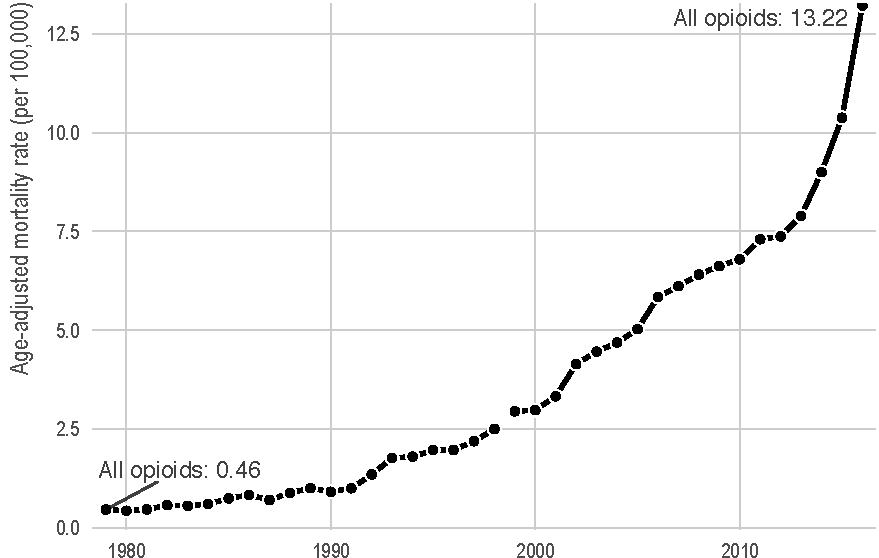
\includegraphics{paa_slides_files/figure-beamer/unnamed-chunk-1-1.pdf}

\end{frame}

\begin{frame}{More than deaths by car accidents or guns}

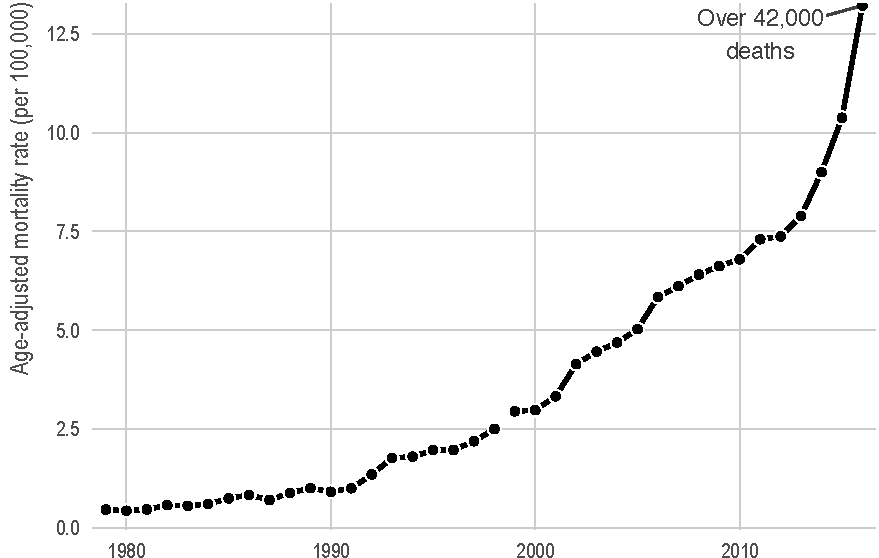
\includegraphics{paa_slides_files/figure-beamer/unnamed-chunk-2-1.pdf}

\end{frame}

\section{Variation in the opioid
epidemic}\label{variation-in-the-opioid-epidemic}

\begin{frame}{Variation by opioid type}

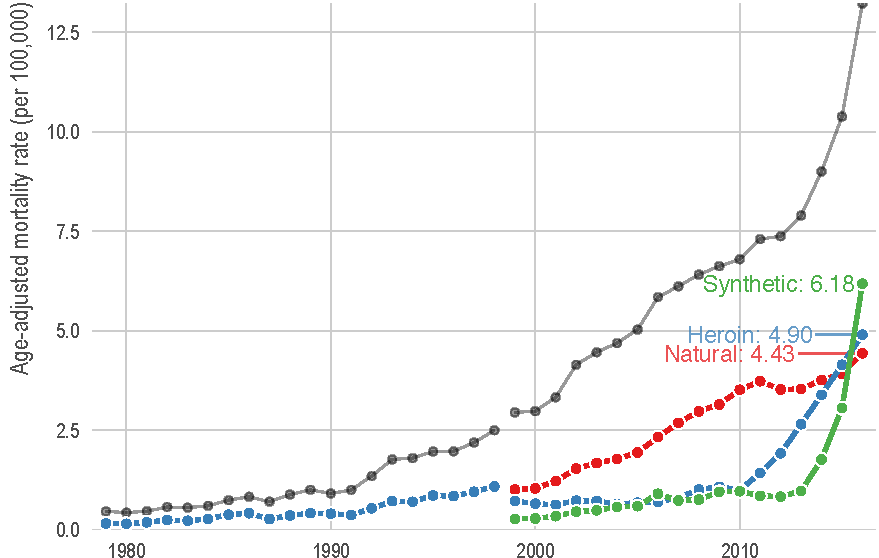
\includegraphics{paa_slides_files/figure-beamer/unnamed-chunk-3-1.pdf}

\end{frame}

\begin{frame}{Variation by race/ethnicity}

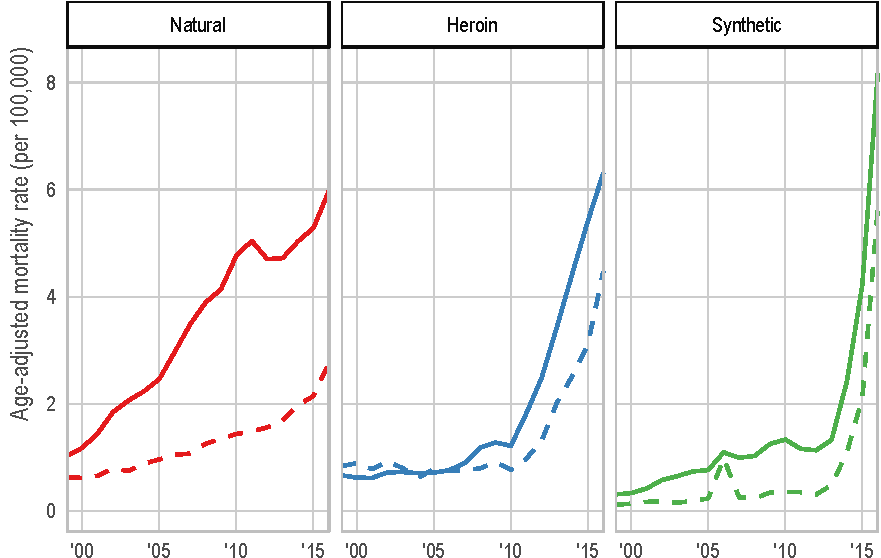
\includegraphics{paa_slides_files/figure-beamer/unnamed-chunk-4-1.pdf}

\end{frame}

\begin{frame}{Variation by state}

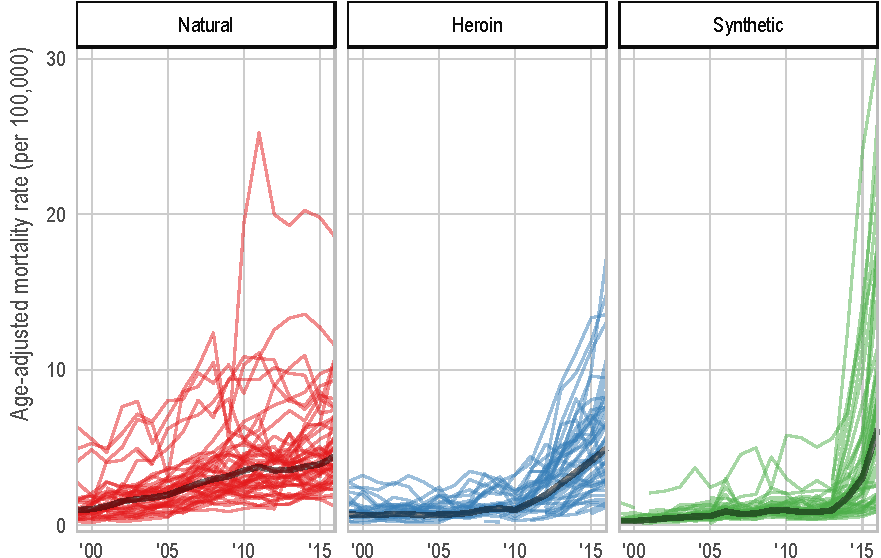
\includegraphics{paa_slides_files/figure-beamer/unnamed-chunk-5-1.pdf}

\end{frame}

\begin{frame}{Aims of the paper}

\begin{enumerate}[<+->]
\def\labelenumi{\arabic{enumi}.}
\tightlist
\item
  Systematically describe the opioid epidemic across geography (state),
  race/ethnicity, and opioid type.

  \begin{itemize}[<+->]
  \tightlist
  \item
    The epidemic over time (1999--2016)
  \item
    The \emph{current} epidemic in terms of both mortality rate and rate
    of increase
  \end{itemize}
\item
  Identify ``epidemic hotspots'' --- areas with high mortality and rapid
  increases
\end{enumerate}

\end{frame}

\begin{frame}{Data / Methods}

\begin{enumerate}[<+->]
\def\labelenumi{\arabic{enumi}.}
\tightlist
\item
  Multiple cause of death data from NCHS
\item
  Calculate age-standardized rates by state, race/ethnicity, and opioid
  type
\item
  Joinpoint regression
\end{enumerate}

\end{frame}

\begin{frame}{Example Results: Maryland}

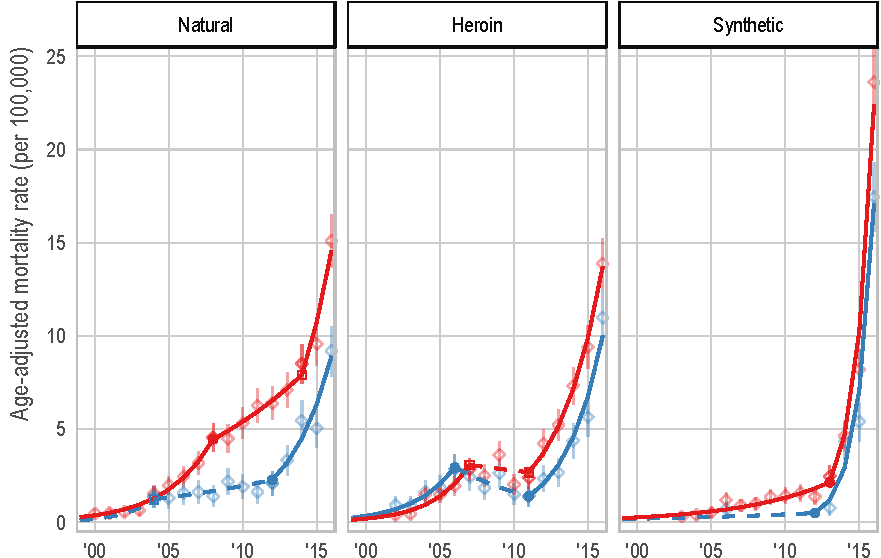
\includegraphics{paa_slides_files/figure-beamer/unnamed-chunk-6-1.pdf}

\end{frame}

\begin{frame}{Example Results: Synthetic Opioids}

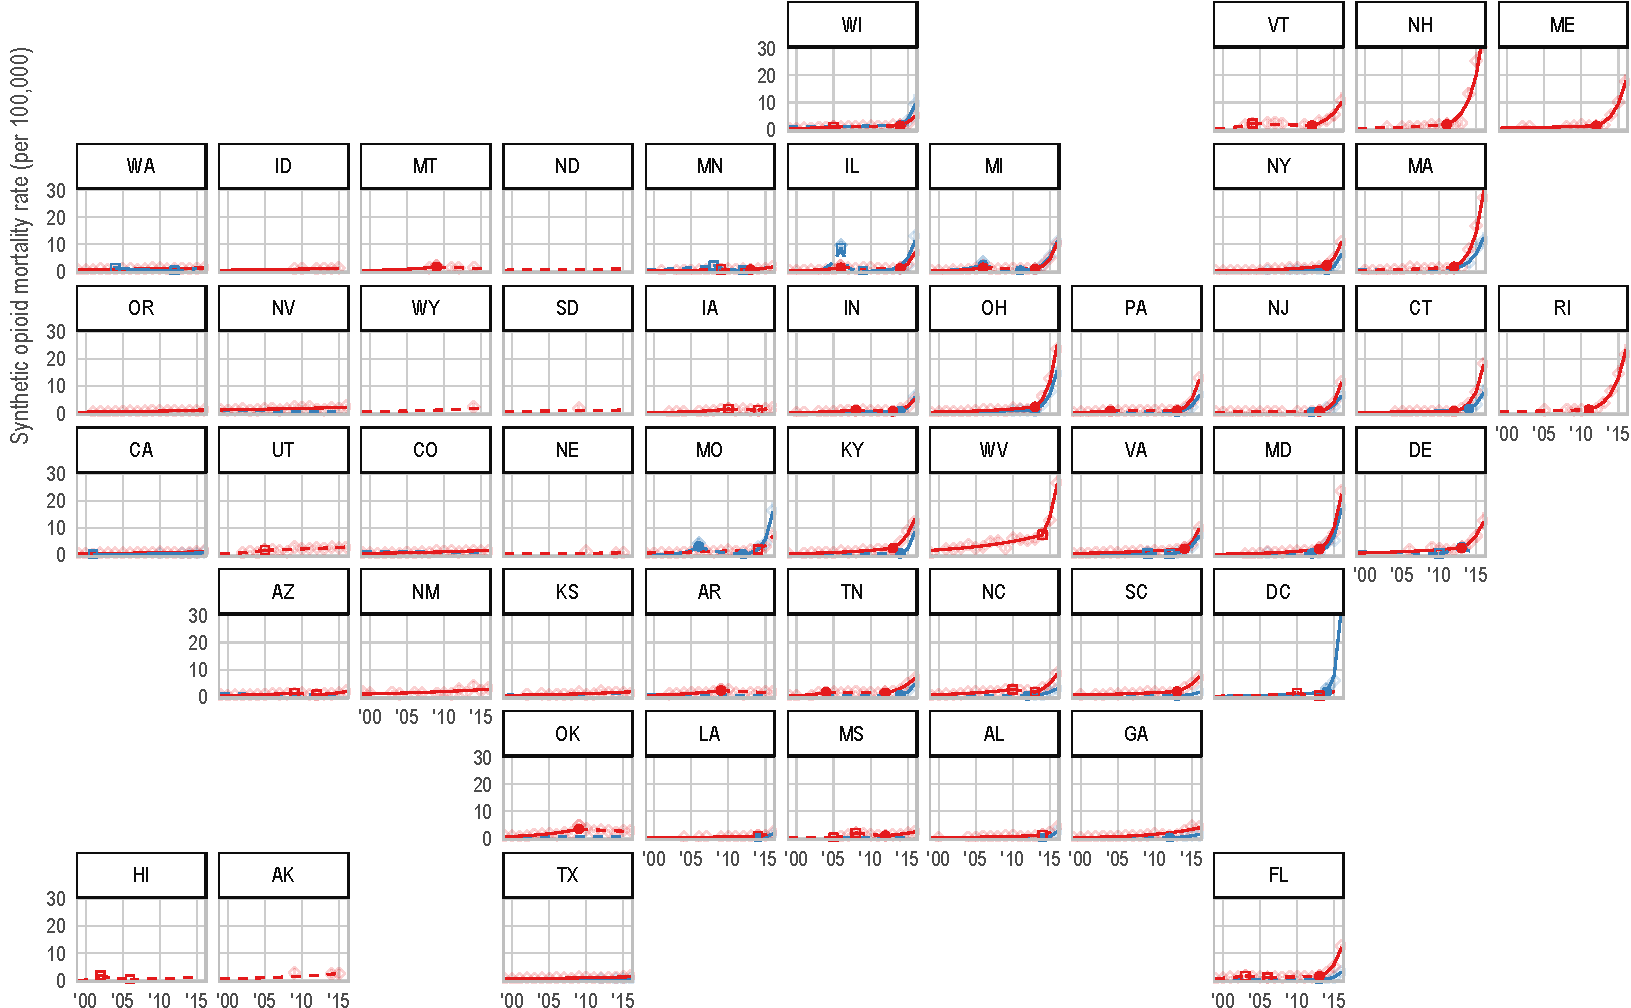
\includegraphics{paa_slides_files/figure-beamer/unnamed-chunk-7-1.pdf}

\end{frame}

\section{Results: Current Epidemic}\label{results-current-epidemic}

\begin{frame}{Current Mortality}

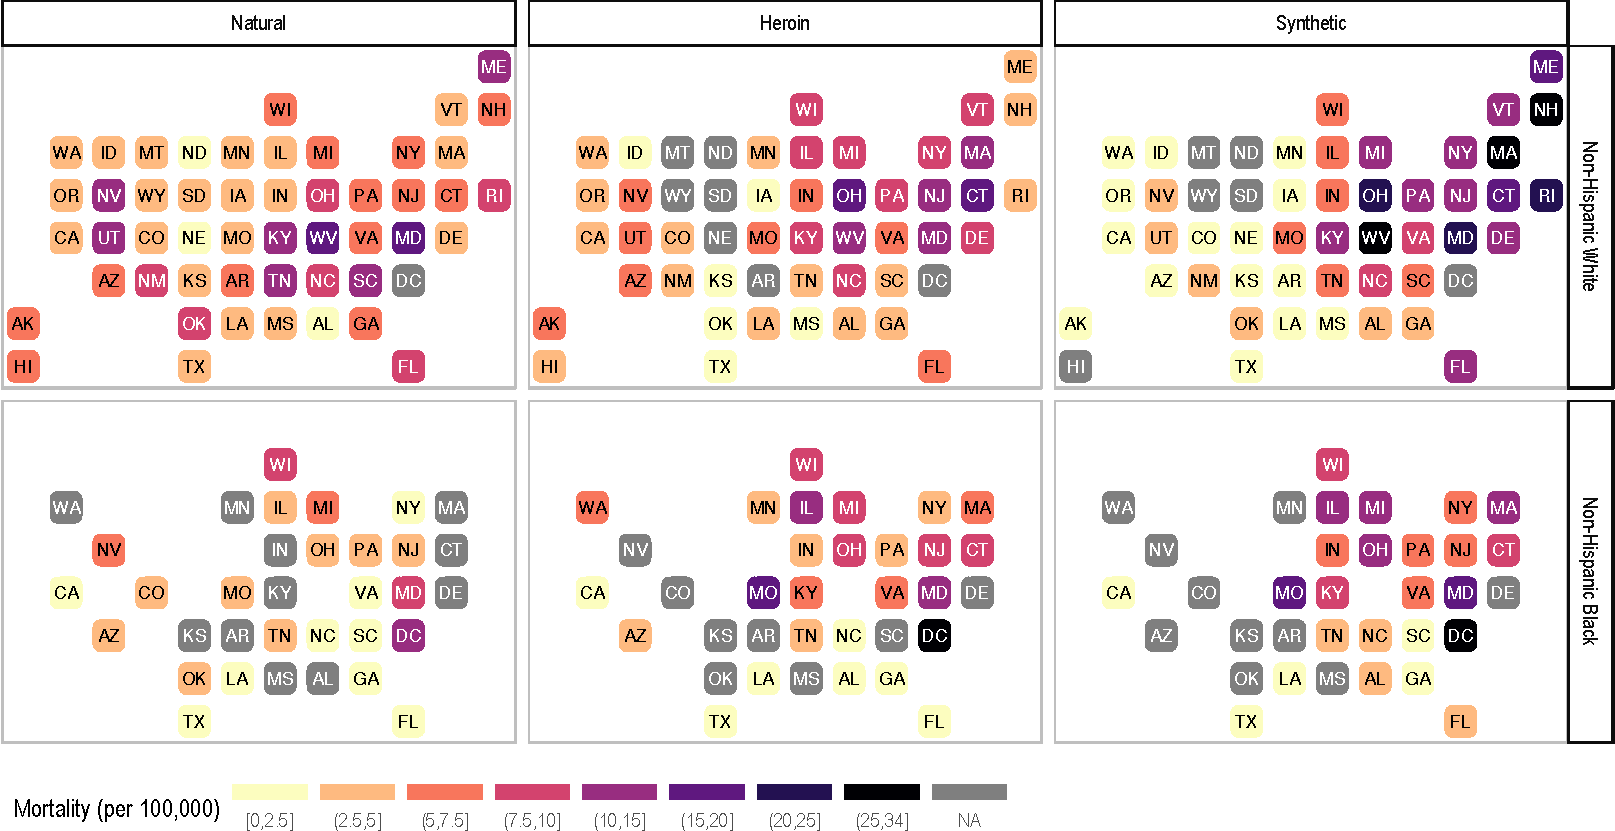
\includegraphics{paa_slides_files/figure-beamer/unnamed-chunk-8-1.pdf}

\end{frame}

\begin{frame}{Current Trajectory}

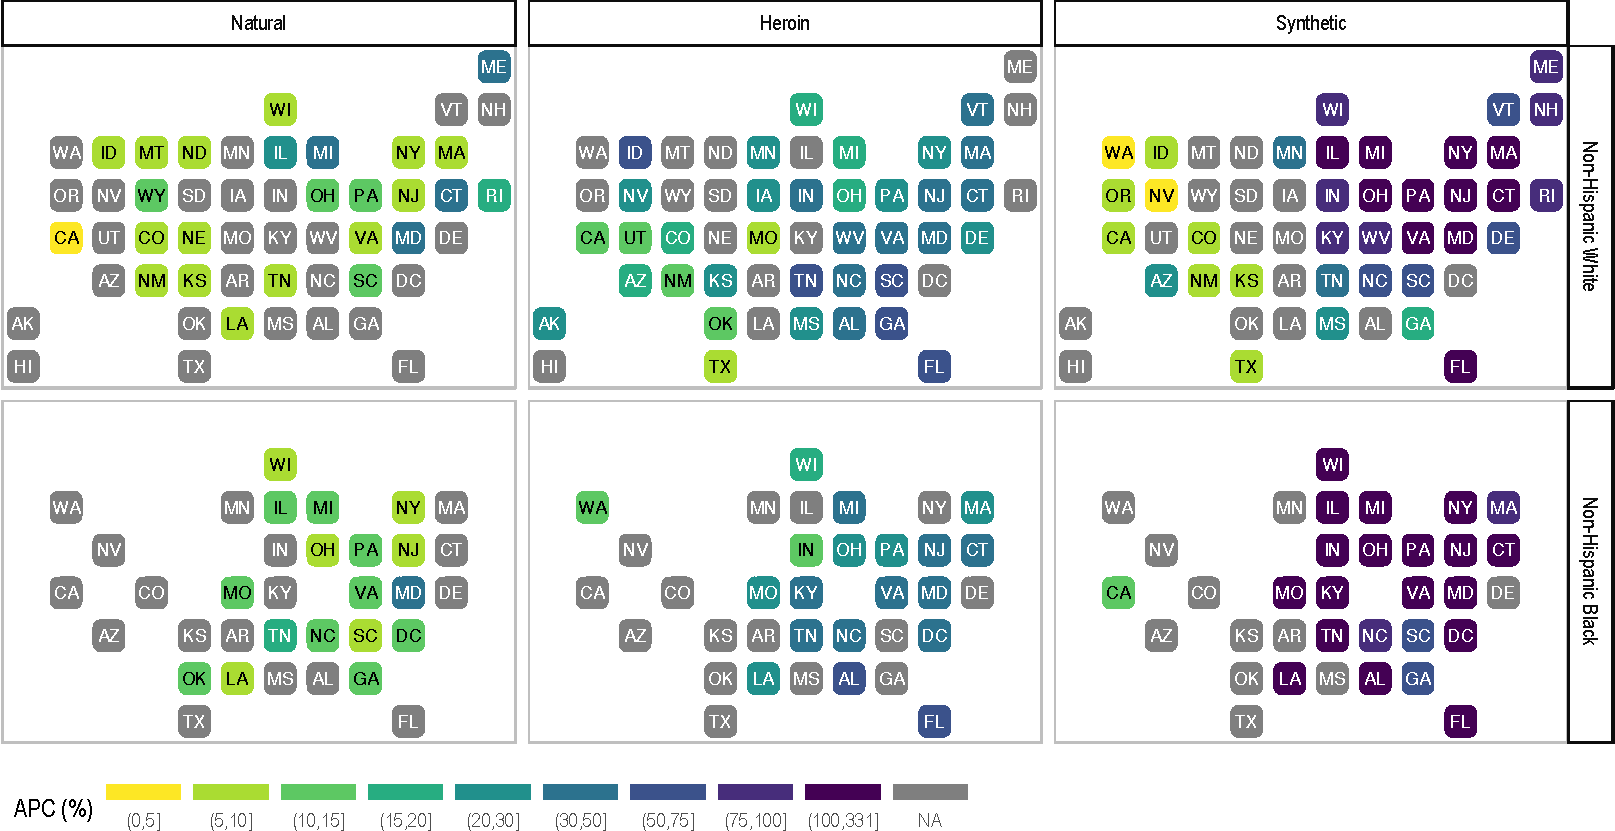
\includegraphics{paa_slides_files/figure-beamer/unnamed-chunk-9-1.pdf}

\end{frame}

\begin{frame}{Epidemic Hotspots}

\begin{center}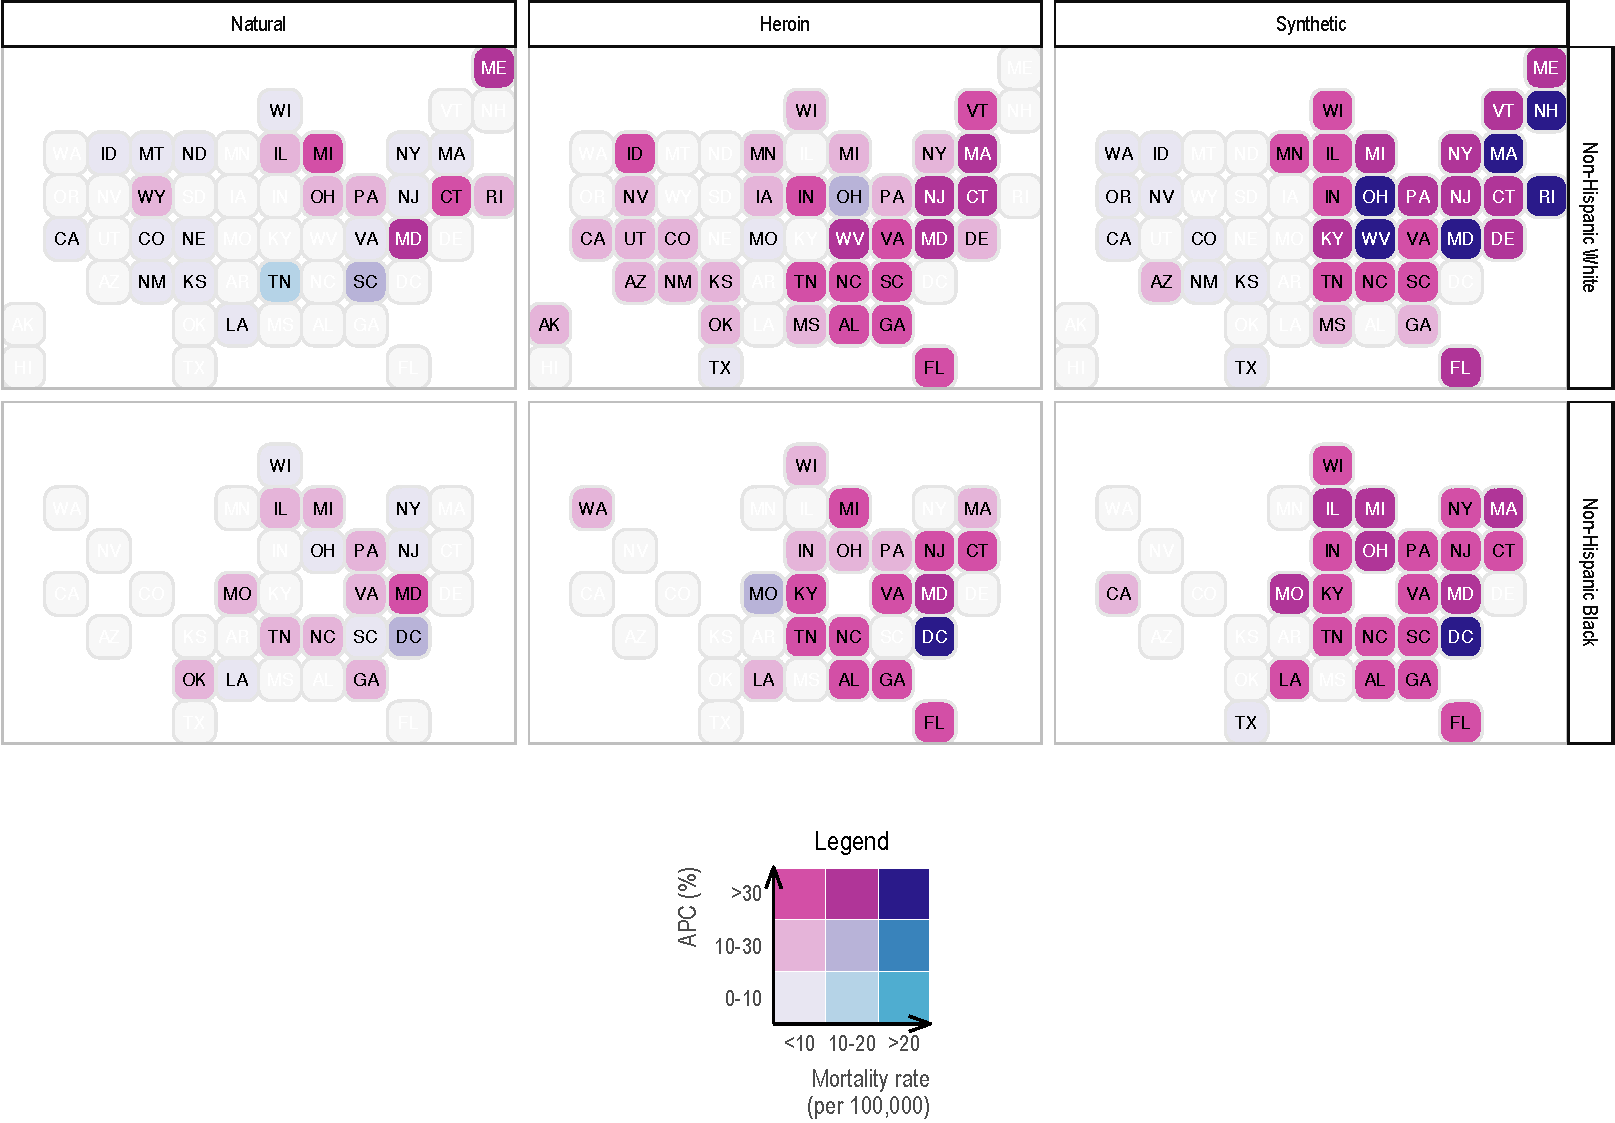
\includegraphics{paa_slides_files/figure-beamer/unnamed-chunk-10-1} \end{center}

\end{frame}

\begin{frame}{Results}

\begin{itemize}[<+->]
\tightlist
\item
  No decreases in opioid mortality over whole time period
\item
  Where there were increases, it is just as bad (or worse) for the black
  population
\item
  Increases are driven by heroin and synthetic opioids in eastern states

  \begin{itemize}[<+->]
  \tightlist
  \item
    Heroin deaths increased 30-34\% per year for both populations
  \item
    Synthetic opioids increased 70\% per year for whites and 150\% for
    blacks
  \end{itemize}
\item
  Synthetic opioids are doubling in 12 states for whites and 18 for
  blacks
\item
  Strong geographical clustering of epidemic hotspots
\end{itemize}

\end{frame}

\begin{frame}{Conclusions}

\begin{itemize}[<+->]
\tightlist
\item
  Interventions must be local and tailored to region, race/ethnicity,
  and opioid type
\item
  Supply-side interventions need to be balanced with harm reduction
  interventions

  \begin{itemize}[<+->]
  \tightlist
  \item
    Syringe exchange programs
  \item
    Medication assisted treatment
  \item
    Increased naloxone access
  \item
    Drug testing on-site and point-of-site
  \item
    Supervised consumption sites
  \end{itemize}
\item
  Surveillance of illicit markets needs to be dramatically improved

  \begin{itemize}[<+->]
  \tightlist
  \item
    Better measurement of potency of drugs
  \item
    Types of drugs
  \item
    Cost and availability
  \end{itemize}
\end{itemize}

\end{frame}

\begin{frame}{Thank you}

\Large

\begin{center}
\textbf{Code and interactive results explorer:} \\ \texttt{https://tiny.cc/paa2018} \newline \newline

 mathewkiang.com | \faGithub: mkiang | \faTwitter: @mathewkiang 

\end{center}

\end{frame}

\begin{frame}{Epidemic Hotspots}

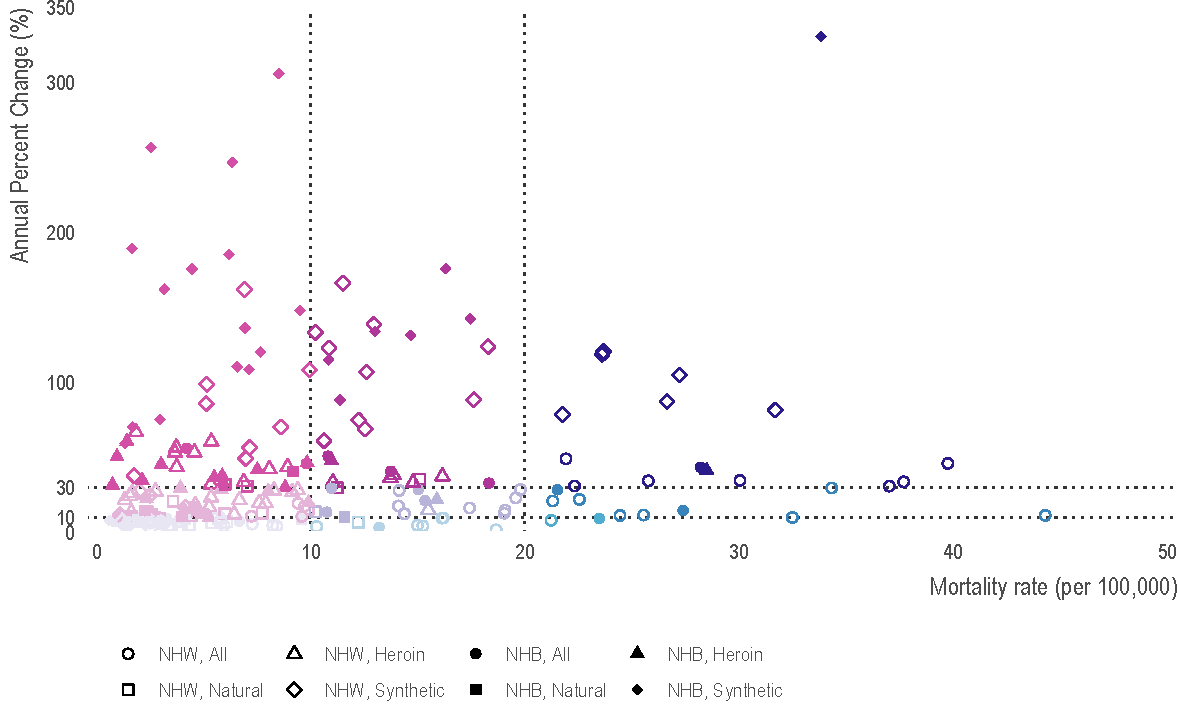
\includegraphics{paa_slides_files/figure-beamer/unnamed-chunk-11-1.pdf}

\end{frame}

\begin{frame}{Average Annual Percent Change}

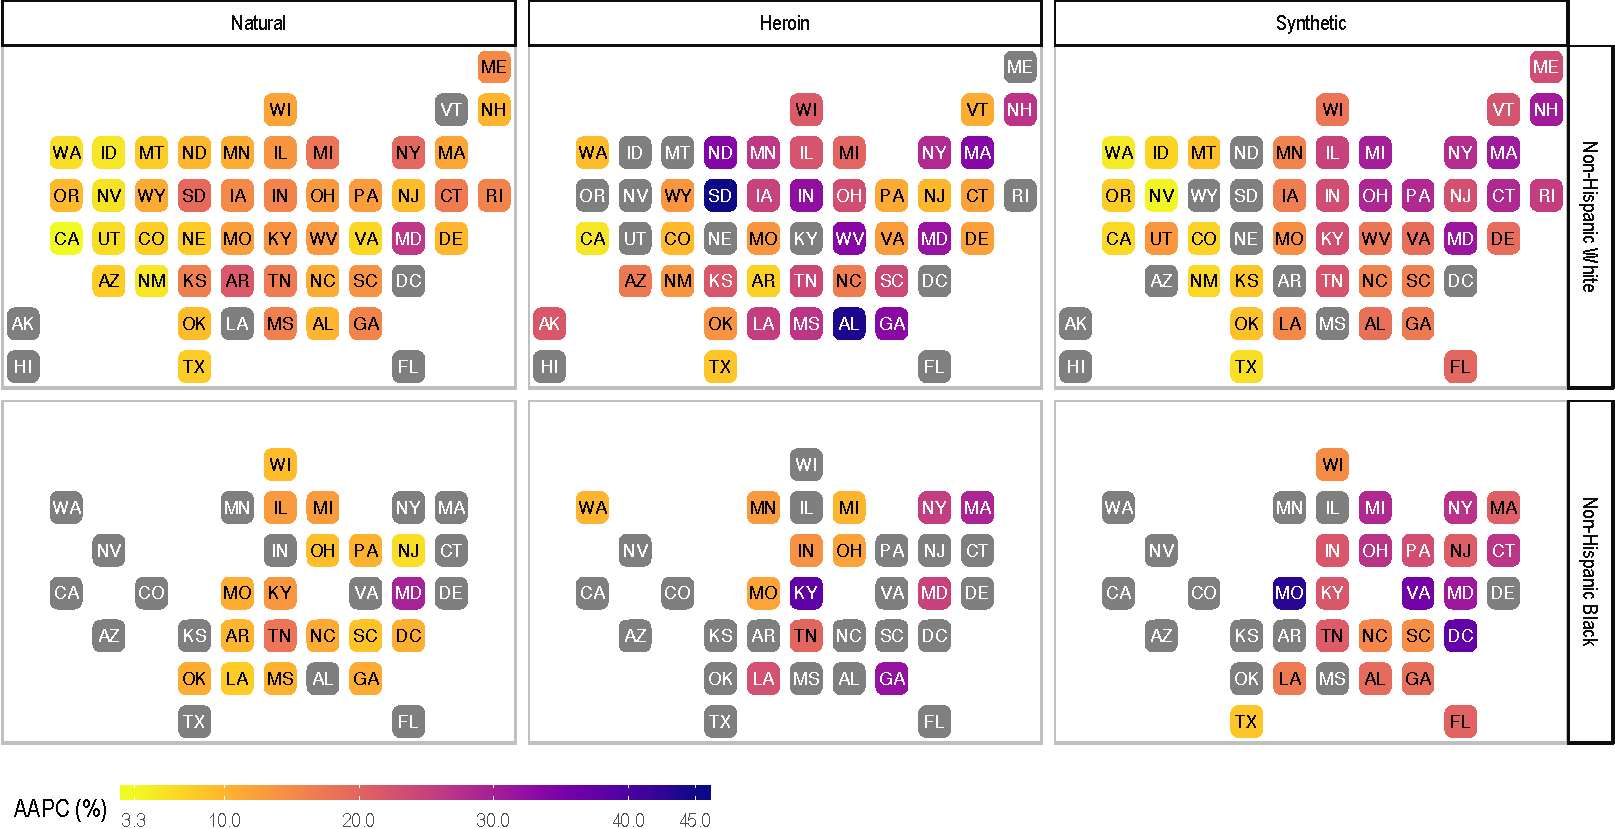
\includegraphics{paa_slides_files/figure-beamer/unnamed-chunk-12-1.pdf}

\end{frame}

\end{document}
